\chapter{Analisis Persoalan dan Rancangan Solusi}

Tujuan utama penulisan bab ini adalah untuk menguraikan rencana penyelesaian masalah tugas akhir yang akan dieksekusi secara utuh pada saat pelaksanaan Tugas Akhir II. Bab ini merupakan bab penutup Laporan Tugas Akhir I yang dapat dipandang sebagai bab yang akan menjembatani perpindahan ke proses pelaksanaan Tugas Akhir II. Pengembangan lebih lanjut dari bab ini dapat menjadi bagian dari bab Deskripsi Solusi pada Laporan Tugas Akhir.

\section{Analisis Persoalan}

\textit{Autoscaler} merupakan salah satu teknologi yang bermanfaat untuk membantu pengelola infrastruktur dalam melakukan \textit{scaling} pada teknologi \textit{container orchestration} seperti Kubernetes. Dengan menggunakan \textit{autoscaler}, pengguna dapat mengatur dan mengontrol (\textit{scaling}) sumber daya dari sekumpulan \textit{pods} dengan otomatis. Pada teknologi \textit{autoscaler} yang paling sederhana, sistem akan secara otomatis melakukan \textit{scaling} apabila suatu metrik melewati ambang batas tertentu. Beberapa \textit{autoscaler} yang paling populer saat ini adalah \textit{horizontal autoscaling} dan \textit{vertical autoscaling} yang melakukan \textit{scaling} berdasarkan metrik sistem seperti utilisasi prosesor, memori serta beban permintaan dalam satuan waktu. Perkembangan dari metode \textit{autoscaling} telah menyediakan pengguna berbagai opsi untuk mengotomasi alokasi sumber daya. Namun, dari semua metode yang sekarang sudah ada, terdapat beberapa kekurangan yang dapat diperbaiki, diantaranya sebagai berikut.

\begin{enumerate}
    \item Terdapat keperluan pengelola untuk melakukan \textit{error and trial} untuk memenuhi standar \textit{quality of service} yang berbentuk \textit{throughput} karena tidak adanya data sebab akibat dari prosesor dan memori pada \textit{throughput}. Terutama apabila permintaan standar spesifik pada operasi tertentu di \textit{Elastic Search}.
    \item \textit{Autoscaler} sederhana umumnya dibuat untuk sesuatu yang sangat umum seperti pemrosesan seperti \textit{web service}, \textit{CRON Job}, dan sebagainya. Hal ini sedikit berbeda jika berkaitan dengan sistem \textit{information retrieval}, karena sistem \textit{information retrieval} memiliki data yang berbeda sehingga kegunaan dan keperluannya menjadi bervariatif.
    \item \textit{Metrics} yang digunakan adalah data \textit{realtime} dan berpatokan dengan sebuah ambang batas sehingga tidak efisien terhadap kinerja sistem yang fluktuatif. Apabila hanya mengandalkan angka ambang batas, ketika sistem melewati angka ambang batas untuk waktu yang sangat singkat, maka sistem akan mencoba untuk melakukan \textit{scaling} yang sebenarnya bisa dianggap tidak perlu jika hanya singkat, \parencite{riset1}.
    \item Setiap pengelola infrastruktur memiliki variabel \textit{cost} dan target kinerja sistem yang berbeda-beda. Toleransi terhadap target kinerja sistem dan \textit{cost} yang berbeda memerlukan \textit{autoscaler} yang dapat dikonfigurasi dengan fleksibel.
    \item \textit{Rolling Update} yang terlalu sering mengharuskan kubernetes memiliki sumber daya minimal sejumlah dua kali lipat. Selain itu, hal ini juga memiliki overhead karena \textit{Elastic Search} perlu melakukan beberapa proses saat dinyalakan.
\end{enumerate}

Pada tugas akhir ini, akan dilakukan penelitian untuk melakukan pengembangan metode \textit{autoscale} yang berjalan diatas Kubernetes yang spesifik untuk mengontrol alokasi sumber daya \textit{Elastic Search}. Dengan melakukan pengembangan tersebut, diharapkan penelitian ini dapat meningkatkan efisiensi \textit{autoscale} pada \textit{Elastic Search} dengan kontrol fleksibel berdasarkan model prediktif berbasis \textit{time series}. Pendekatan prediksi berbasis \textit{time series} dilakukan karena metrik sistem sangat dekat dengan data historis dan korelasi data dengan waktu. Melalui referensi studi literatur yang sudah dilakukan, banyak penelitian yang menggunakan model prediksi dengan \textit{time series} seperti ARIMA, LSTM, dan Bi-LSTM.

% Namun, saat ini kontrol adaptif milik Kubernetes memiliki beberapa kekurangan. Salah satu kekurangan dari kontrol adaptif kubernetes adalah \textit{trigger autoscale} yang didasarkan oleh metriks umum seperti utilisasi memori dan prosesor berdasarkan waktu saat itu. Sedangkan, tidak semua \textit{container} dinyatakan memakai sumber daya komputasi secara efisien jika hanya memakai faktor tersebut sebab tidak semua \textit{container} bergantung hanya pada utilisasi prosesor dan memori. Terkadang ada beberapa fitur pada sebuah \textit{container} yang terus berjalan namun tidak terpakai atau disimpan pada \textit{cache} namun tidak dipakai. Semuanya kembali lagi kepada isi dari sebuah \textit{container} serta penggunaannya. Selain dari hal tersebut, kubernetes juga hanya memakai data \textit{metrics} yang sedang berlangsung. Sehingga, kubernetes tidak dapat memprediksi kebutuhan \textit{resource} pada waktu yang akan datang melalui pola penggunaan. Hal ini akan menjadi acuan untuk meningkatkan efisiensi \textit{autoscale} dari kubernetes terutama pada \textit{Elastic Search} melalui adaptif kontrol dengan model prediktif berbasis \textit{time series}.

\section{Analisis Solusi}

Untuk melakukan penelitian pengembangan kontrol adaptif tersebut, dilakukan pemetaan masalah, penanganan serta kebutuhan untuk melakukan penanganan tersebut.

\subsection{Pemetaan Masalah dan Penanganan}
\label{sec:pemetaan-masalah}
Masalah-masalah yang ada akan dipetakan dengan penanganan yang akan dilakukan. Pemetaan masalah dan penanganan dapat dilihat pada Tabel \ref{tab:pemetaan-masalah}.

\begin{table}[h]
    \caption{Tabel Pemetaan Masalah dan Penanganan}
    \vspace{0.25cm}
    \begin{center}
        \begin{tabular}{|c|p{2.5in}|p{2.5in}|}
            \hline
            Nomor & Masalah & Penanganan \tabularnewline
            \hline
            1 &
            Kubernetes tidak bisa melakukan kontrol adaptif berdasarkan variabel spesifik pada suatu kontainer. &
            Kontrol adaptif harus spesifik untuk suatu jenis kontainer, pada tugas akhir ini, akan berfokus pada \textit{Elastic Search}. \tabularnewline
            2 &
            \textit{Metrics} yang digunakan adalah data \textit{realtime} sehingga jika ada turbulensi akan mengurangi efisiensi dan performa. &
            Kontrol adaptif memakai model prediksi berbasis \textit{time series} sehingga dapat melihat korelasi dengan data yang ada di masa lalu.\tabularnewline
            3 & Terdapat keperluan untuk \textit{error and trial} untuk memenuhi standar \textit{quality of service} yang berbentuk \textit{throughput} karena tidak memiliki data sebab akibat dari prosesor dan memori pada \textit{throughput}. &
            Menambah variabel \textit{throughput} untuk melakukan kontrol adaptif.
            \tabularnewline
            4 & \textit{Rolling Update} yang terlalu sering mengharuskan kubernetes memiliki sumber daya minimal sejumlah dua kali lipat. &
            Menggunakan \textit{In-Place Update of Pod Resources} \tabularnewline
            5 & \textit{Quality of service} dan toleransi kepada \textit{tradeoff} antara efisiensi dan \textit{cost} dapat berbeda antara pengguna. &
            Kontrol adaptif harus memiliki ruang untuk pengguna membuat aturan terhadap kontrol adaptif.\tabularnewline
            \hline
        \end{tabular}
    \end{center}
    \label{tab:pemetaan-masalah}
\end{table}

\subsection{Rencana Penanganan Masalah dan Analisis Kebutuhan}

Masalah sudah dipetakan pada bagian \ref{sec:pemetaan-masalah} dan penanganan secara kasar telah dirancangkan. Dalam melakukan penanganan masalah tersebut, diperlukan beberapa kebutuhan yang akan dijelaskan pada bagian ini.

\begin{enumerate}
    \item \textbf{Menambah variabel untuk melakukan kontrol adaptif yang spesifik pada \textit{throughput} dan spesifikasi \textit{Elastic Search}}
    
    Kebutuhan ini secara umum bisa didapatkan melalui \href{https://www.elastic.co/guide/en/elasticsearch/reference/current/cluster-nodes-stats.html}{\textit{Node Stats API}}. Untuk variabel yang akan ditarik, akan digunakan \textit{metrics response time} dari setiap operasi yang ada di \textit{Elastic Search} seperti \textit{Index, Get, Query, Fetch, Bulk, Refresh, Scroll, Suggest} dan \textit{Flush} serta \textit{metrics} umum seperti utilisasi prosesor serta memori.

    \item \textbf{Membuat model prediksi berbasis \textit{time series}}
    
    Kebutuhan ini bisa dilakukan dengan beberapa pendekatan seperti ARIMA, SARIMA, LSTM serta variasi seperti ARIMA. Dalam tugas akhir ini, akan digunakan ARIMA untuk melakukan prediksi \textit{metrics} yang ada. Alasan menggunakan ARIMA adalah karena ARIMA merupakan model yang sederhana dan mudah untuk diimplementasikan. Selain itu, ARIMA juga merupakan model yang cukup baik untuk melakukan prediksi \textit{time series} yang memiliki \textit{trend} dan \textit{seasonality}. Ditambah, variasi dari ARIMA memiliki masalah ketika data memiliki standar deviasi rendah, contohnya adalah VARMAX atau \textit{Vector Auto Regressive Moving Average with Exogenous Regressors}. Meskipun dengan satu model VARMAX, koneksi antara variabel juga bisa ditentukan, namun ARIMA juga sudah cukup baik untuk memprediksi variabel-variabel secara terpisah.

    \item \textbf{Menggunakan \textit{In-Place Update of Pod Resources}}

    \textit{In-Place Update of Pod Resources} merupakan fitur baru yang dikembangkan oleh Kubernetes yang bertujuan untuk dapat mengubah ukuran pod secara dinamis tanpa melakukan \textit{restart}. Fitur ini baru saja dicoba diimplementasikan dan dipublikasikan dengan status \textit{alpha testing} sejak 12 Mei 2023, \parencite{kubeinplaceupdate}. Fitur ini layak diteliti untuk melakukan \textit{resizing} tanpa melakukan \textit{restart}. Sebagai catatan, saat tugas akhir ini dikerjakan, fitur ini masih memiliki banyak keterbatasan dan masalah yang tertulis pada blog kubernetes maupun belum tertulis.

    \item \textbf{Menerapkan \textit{rule} untuk kontrol adaptif yang ditetapkan pengguna}
    
    Kebutuhan ini bisa dipenuhi dengan membuat bahasa \textit{scripting} yang simpel untuk mengekspresikan \textit{rule}/kondisi yang ingin ditetapkan pengguna. Prediksi dan waktu prediksi suatu variabel dapat ditentukan oleh pengguna melalui bahasa \textit{scripting} sehingga pengguna dapat menggunakan model prediksi dengan leluasa. Selain itu, terdapat juga beberapa konfigurasi sistem yang dapat dikonfigurasi oleh pengguna agar dapat menyesuaikan sistem kontrol adaptif dengan kebutuhan.

\end{enumerate}

\section{Rancangan Solusi}
Dengan segala kebutuhan yang sudah dianalisis, maka akan dibuat beberapa komponen penyusun sistem yang bisa dilihat pada gambar \ref{fig:rancangan-sistem}. Rencananya, sistem kontrol adaptif akan dikembangkan dari luar kubernetes cluster sedangkan \textit{Elastic Search} itu sendiri diletakkan didalam kubernetes. Integrasi dengan API \textit{Elastic Search} akan melalui \textit{service} yang disediakan kubernetes sedangkan untuk mengontrol kubernetesnya sendiri akan digunakan \textit{Kubernetes Client Library}.

\begin{figure}[h]
    \centering
    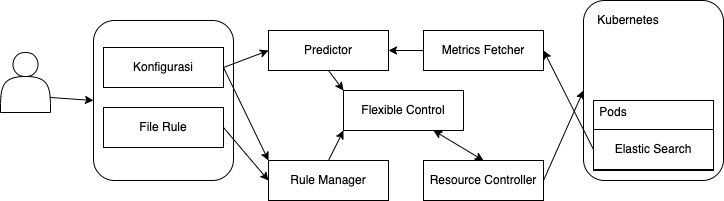
\includegraphics[width=0.8\textwidth]{chapter-3/rancangan.png}
    \caption{Rancangan Komponen Penyusun Sistem}
    \label{fig:rancangan-sistem}
\end{figure}

Pada gambar \ref{fig:rancangan-sistem}, sistem kontrol adaptif tersusun dari beberapa komponen, diantaranya sebagai berikut.

\begin{enumerate}
    \item \textbf{Konfigurasi dan \textit{File Rule}}
    
    Konfigurasi dan \textit{File Rule} akan berinteraksi langsung dengan pengguna. Konfigurasi akan dibaca oleh mayoritas komponen sebagai pengaturan terhadap sistem sedangkan file rule yang di\textit{parse} oleh \textit{rule manager} untuk mengatur trigger dari \textit{resource controller} melakukan kontrol adaptif terhadap alokasi sumber daya.

    \item \textbf{Kubernetes dan \textit{Elastic Search}}
    
    \textit{Elastic Search} akan diletakkan pada sebuah \textit{pods} di dalam sebuah \textit{cluster Kubernetes}. Dibuatkan sebuah \textit{service} agar \textit{Elastic Search} dapat diakses dari luar \textit{cluster}.
    
    \item \textbf{\textit{Predictor}}
    
    \textit{Predictor} akan berisikan model ARIMA untuk setiap variabel yang telah ditentukan. Model-model ini akan digunakan untuk memprediksi nilai variabel pada waktu selanjutnya sesuai permintaan \textit{rule manager}. Karena setiap rule mungkin untuk memiliki keperluan data untuk waktu prediksi yang berbeda.

    \item \textbf{\textit{Metrics Fetcher}}
    
    Komponen \textit{Metrics Fetcher} bertugas untuk menembak \href{https://www.elastic.co/guide/en/elasticsearch/reference/current/cluster-nodes-stats.html}{\textit{Node Stats API}} yang dimiliki oleh \textit{Elastic Search} dan meneruskannya kepada komponen \textit{Predictor} untuk melatih model.

    \item \textbf{\textit{Rule Manager}}
    
    Komponen \textit{Rule Manager} akan melakukan parsing terhadap file rule yang telah diisi oleh pengguna dan mengatur \textit{trigger}. Selain itu, komponen ini akan memberikan informasi tentang waktu prediksi yang diperlukan berdasarkan \textit{rule} yang telah dibuat oleh pengguna.

    \item \textbf{\textit{Resource Controller}}
    
    Komponen \textit{Resource Controller} akan memanfaatkan \textit{Kubernetes Client Library} untuk mengubah spesifikasi \textit{deployment} sehingga alokasi sumber daya dapat berubah.

    \item \textbf{\textit{Adaptive Control}}
    
    Komponen \textit{Adaptive Control} adalah komponen \textit{high-level} yang akan mengintegrasikan dan mengkolaborasikan komponen-komponen yang disebutkan sebelumnya.
\end{enumerate}